
\documentclass[11pt,a4paper,openany]{report}
\usepackage[T1]{fontenc}
\usepackage[utf8]{inputenc}
\usepackage{lmodern}
\usepackage{microtype}
\usepackage{amsmath,amssymb,amsthm,mathtools,bm}
\usepackage{booktabs,array,longtable,tabularx}
\usepackage{xcolor}
\usepackage[margin=22mm,headheight=23pt]{geometry}
\usepackage{enumitem}
\usepackage{fancyhdr}
\usepackage{fancyvrb}
\usepackage{graphicx}
\usepackage{url}
\usepackage{xurl}
\usepackage{hyperref}
\definecolor{finblue}{HTML}{1F5A99}
\definecolor{fingreen}{HTML}{19733A}
\definecolor{finorange}{HTML}{D55E00}
\definecolor{finred}{HTML}{A61B1B}
\definecolor{finviolet}{HTML}{6A3D9A}
\definecolor{fingray}{HTML}{4D4D4D}

\hypersetup{
  unicode=true,
  colorlinks=true,
  linkcolor=finblue,
  citecolor=fingreen,
  urlcolor=finblue,
  pdftitle={FIN Research Programs P295--P308},
  pdfauthor={Krzysztof Żuchowski},
  pdfsubject={Legacy physics, strict spectral completion, and physical-role transfer},
  pdfkeywords={FIN, legacy kernel, strict kernel, positive Laplace mixture, Bernstein function, Naimark dilation, scale gauge, role transfer}
}
\pagestyle{fancy}
\fancyhf{}
\fancyhead[L]{\small FIN Programs P295--P308}
\fancyhead[R]{\small Release 10.27}
\fancyfoot[C]{\thepage}

\setlength{\parindent}{0pt}
\setlength{\parskip}{0.55em}
\setlist{nosep,leftmargin=2em}
\setcounter{tocdepth}{2}
\setcounter{secnumdepth}{3}
\emergencystretch=3em
\newcommand{\one}{\bm 1}
\newcommand{\C}{\mathbb C}
\newcommand{\R}{\mathbb R}
\newcommand{\Z}{\mathbb Z}
\newcommand{\statusProven}{\textcolor{fingreen}{[Proven]}}
\newcommand{\statusStrong}{\textcolor{finblue}{[Strong evidence]}}
\newcommand{\statusModerate}{\textcolor{finviolet}{[Moderate evidence]}}
\newcommand{\statusWeak}{\textcolor{fingray}{[Weak evidence]}}
\newcommand{\statusSpeculative}{\textcolor{finorange}{[Speculative]}}
\newcommand{\statusRefuted}{\textcolor{finred}{[Refuted]}}

\begin{document}
\hypersetup{pageanchor=false}
\begin{titlepage}
\centering
\vspace*{7mm}
{\Large\bfseries FIN --- Release 10.27\par}
\vspace{9mm}
{\Huge\bfseries Research Programs P295--P308\par}
\vspace{6mm}
{\Large Legacy physics revisited:\\
positive path mixtures, strict spectral completion,\\
and physical-role transfer\par}
\vspace{13mm}
{\Large Krzysztof \.Zuchowski\par}
\vspace{2mm}
{\normalsize Independent Researcher --- Fractal Information Theory Project\par}
\vspace{2mm}
{\normalsize ORCID:
\href{https://orcid.org/0009-0002-0909-3613}{0009-0002-0909-3613}\par}
\vspace{7mm}
{\large 30 July 2026\par}
{\normalsize Publication --- Preprint; Version 1.0.0\par}
\vfill
\begin{minipage}{0.92\textwidth}
\small
\textbf{Central result.}
The legacy hyperbolic envelope is an exact positive mixture of exponential
distance attenuations.  The strict envelope, phase signs, and spectral order
lie outside positive fixed-phase and monotone scalar-completion classes.

\medskip
\textbf{New boundary objects.}
The Typed Legacy--Strict Completion Span and the Role-Transfer Certificate
separate mathematical completion from physical interpretation.  No historical
electroweak, electromagnetic, or gravity role currently passes the
certificate.

\medskip
\textbf{Repository.}
\url{https://github.com/hyconiek/Fractal-Nadsoliton-Theory}

\textbf{License.} CC BY 4.0.
\end{minipage}
\vfill
\end{titlepage}
\hypersetup{pageanchor=true}
\pagenumbering{roman}
\chapter*{Publication statement}
\addcontentsline{toc}{chapter}{Publication statement}
This monograph reports all executed Programs P295--P308 and recommends
Programs P309--P322.  It corrects historical legacy-kernel calculations,
preserves the legacy/strict split, and keeps mathematical proof, synthetic
evidence, scoped refutation, and missing external evidence distinct.
QW-2191, full bridge completion, physical-role transfer, dimensional
emergence, laboratory validation, \(L_{\rm total}\), and Theory-of-Everything
closure remain open or blocked.

\tableofcontents
\clearpage
\pagenumbering{arabic}

\chapter*{Confidence convention}
\addcontentsline{toc}{chapter}{Confidence convention}

\begin{itemize}
\item 
\textbf{\statusProven{}} --- an analytic identity, exact finite theorem, or machine-checked statement in the explicitly declared class.

\item 
\textbf{\statusStrong{}} --- a reproducible numerical or synthetic audit with frozen inputs, controls, metrics, and stop rules.

\item 
\textbf{\statusModerate{}} --- a robust result that still depends on an additional equivalence, source, or modeling assumption.

\item 
\textbf{\statusSpeculative{}} --- a proposed object or research direction without a sufficient proof.

\item 
\textbf{\statusRefuted{}} --- an explicit counterexample or no-go theorem in the declared class.

\item 
\textbf{[Blocked by external evidence]} --- the executable gate was reached, but independent laboratory data, custody, calibration, or preregistration were absent.

\end{itemize}

A mathematical proof is not evidence that nature realizes its hypotheses.

\chapter{Executive summary}

Programs P295--P308 were executed as a deliberately asymmetric comparison: the historical legacy kernel was reconstructed together with its old connections to physical constants, while the strict kernel was treated as the current finite spectral operator. The kernels were not silently identified, and no historical physical role was transferred to strict.

The central conclusion is:

\begin{quote}\itshape
The old legacy research contains a mathematically meaningful attenuation mechanism, but its maps to electroweak, electromagnetic, gravitational, and Planck-scale physics do not factor through a proved operator observable. The strict kernel cannot be obtained from that attenuation mechanism by positive damping, unchanged phase, or monotone scalar functional calculus. A viable bridge must therefore be typed, non-scalar, operationally testable, and separately equipped with a physical-role certificate.

\end{quote}

The reconstructed legacy attenuation

\[
h_L(d)=\frac{1}{1+\beta d}
\]

has the exact representation

\[
h_L(d)
=
\int_0^\infty e^{-u}e^{-\beta d u}\,du.
\]

It is therefore a positive Laplace mixture of exponential distance attenuations. \textbf{\statusProven{}}

The strict attenuation

\[
h_S(d)=\frac{1}{1+d^{1.8}}
\]

is not completely monotone: its second derivative is negative for sufficiently small positive \(d\). Hence it cannot be generated by the same positive distance-mixture mechanism. The unchanged legacy phase also has the wrong sign at four of the six nonzero \(Z_{12}\) distances. The best positive fixed-phase fit has relative residual \(0.48169\). \textbf{[Proven scoped no-go]}

The obstruction persists at operator level. Scalar complement completions force spectral flat bands with multiplicity incompatible with the strict generator. Moreover, the absolute-value-repaired legacy generator and the strict generator have 32 Fourier-mode order inversions. Every Bernstein function is increasing, so no monotone scalar subordination

\[
A_S=\Phi(A_{L,\lvert\cdot\rvert})
\]

exists in the tested class. \textbf{[Proven scoped no-go]}

The historical physical formulas also fail a modern provenance test.

\begin{itemize}
\item 
The number \(\sin^2\theta_W=\alpha_{\rm geo}/12=\ln2/3\) is a conditional evaluation of an assumed map; the factor \(12\) is not obtained from a strict representation, action, or operator observable.

\item 
The historical expression \[
  \alpha_{\rm EM}^{-1}
  =
  \frac{\alpha_{\rm geo}}{2\beta_{\rm tors}}
  (1-\beta_{\rm tors})
  \] is highly sensitive to \(\beta_{\rm tors}\), omits the phase factor invoked at the start of its old argument, and is not invariant under a change of distance coordinate.

\item 
The hierarchy \(G_{\rm eff}/G_0=\beta_{\rm tors}^N\) does not independently predict \(N\); the historical calculation recovers \(N=19.5\) from a target hierarchy and then rounds to \(20\), changing the result by a factor ten.

\item 
Planck-scale chains import dimensional SI anchors. A dimensionless kernel can transport a supplied scale but does not create a length, time, mass, or action unit.

\end{itemize}

These are not objections to using the old formulas as benchmark hypotheses. They are proofs that the formulas are not yet consequences of the kernel.

P295--P308 also produced constructive results:

\begin{enumerate}
\item 
Four shared probes increase the local Stieltjes inverse rank from \(6\) to \(15\) and reduce median pole error at relative noise \(10^{-4}\) from \(0.496\) to \(0.150\), although uniform stability is still absent.

\item 
Lean 4.28 machine-checks the general logical theorem behind staged minimization, and 400 exact rational SPD Schur witnesses agree.

\item 
The strict six-effect current POVM compiles into an exact \(72\times72\) complex-unitary Givens mesh. The exact reconstruction error is \(2.07\times10^{-15}\); \(10^{-3}\)-radian parameter quantization gives maximum effect error \(1.16\times10^{-3}\).

\item 
A supplied hidden-rate process has conditional mutual information \(0.0010569\) nat, whereas the homogeneous Markov process has zero within \(4.1\times10^{-17}\).

\item 
A joint five-parameter synthetic detector design has full Fisher rank; the gradient RMSE is \(0.00906\).

\item 
The strict fingerprint map is locally rank five. Its rare small-ball probability therefore has leading exponent \(5\); importance sampling gives exponent \(5.217\) over the tested finite range.

\item 
Three exact observation times cannot distinguish homogeneous strict heat flow from a positive time-warped generator; off-grid predictions differ.

\item 
Synthetic interventions raise a hypothetical bridge-coordinate design rank from \(4\) to \(6\), but the coordinate and its law were supplied and are not discoveries about nature.

\item 
The strict heat/\allowbreak{}Gibbs family possesses a scale orbit, while the old electromagnetic and gravity role formulas fail the corresponding coordinate-gauge test.

\item 
A free torsor has no invariant point. Pointing makes an equivariant map unique only after the point is supplied.

\end{enumerate}

No independent P241 event bundle or certified hardware reservoir record was accepted. P242 was not run on invented data. No result closes QW-2191, the full legacy-to-strict bridge, physical-role transfer, a dimensional unit, \(L_{\rm total}\), Standard Model dynamics, general relativity, laboratory validation, or a Theory of Everything.

\begin{figure}[htbp]
\centering
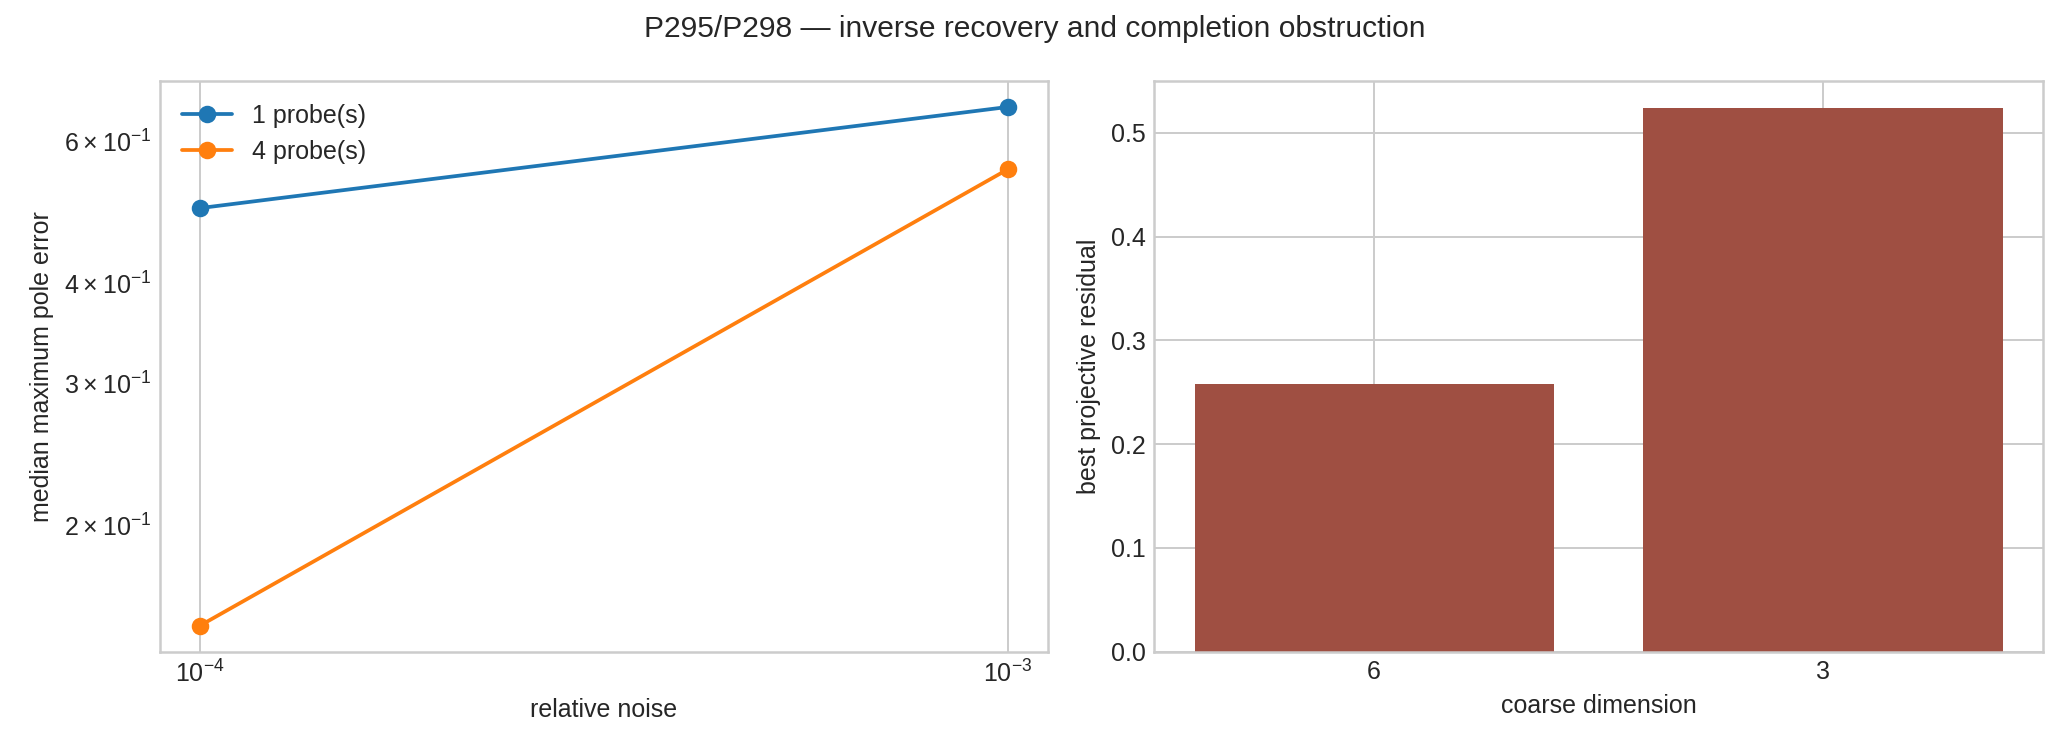
\includegraphics[width=0.97\textwidth]{FIN_Programs_295_308_Figures/p295_p298_inverse_completion.png}
\caption{Multi-probe inverse recovery and the scalar/Bernstein completion obstruction.}
\end{figure}

\chapter{Scope, ontology, and kernel split}

The internal ontology retained in this release is

\[
\text{nadsoliton}
\longrightarrow
\text{light}
\longrightarrow
\text{matter}
\longrightarrow
\text{emergent observer}.
\]

The nadsoliton is treated within FIN as primordial information in a solitonic state. No additional informational layer is inserted below it. This ontology does not by itself define a laboratory observable.

The historical/\allowbreak{}intermediate legacy kernel is

\[
K_L(d)
=
\alpha_{\rm geo}
\frac{\cos(\omega_Ld+\phi_L)}
{1+\beta_{\rm tors}d},
\]

with the canonical historical tuple

\[
\alpha_{\rm geo}=4\ln2,\qquad
\omega_L=\frac{\pi}{4},\qquad
\phi_L=\frac{\pi}{6},\qquad
\beta_{\rm tors}=0.01.
\]

The strict working kernel is

\[
K_S(d)
=
\frac{\cos(\omega_Sd+\phi_S)}
{1+d^\eta},
\qquad
\omega_S=0.18575,\quad
\phi_S=0.16250,\quad
\eta=1.8.
\]

On \(Z_{12}\), its adjacency \(W_S\) and generator are

\[
(W_S)_{xy}=K_S(d(x,y)),
\qquad
A_S=\operatorname{diag}(W_S\mathbf1)-W_S.
\]

The certified finite facts include

\[
A_S=A_S^\ast,\qquad
A_S\mathbf1=0,\qquad
A_S\succeq0,
\]

with one zero mode and spectral gap

\[
\gamma=0.7541211542070796.
\]

The legacy kernel is an intermediate bridge object, not a co-equal final kernel. The strict kernel may be described as a completed/\allowbreak{}enriched continuation only through explicit completion evidence. Neither kernel may silently inherit the other kernel's physical roles.

\chapter{Reconstruction of the historical legacy-to-physics chain}

\section{What the old construction actually establishes}

The historical documentation begins with

\[
D_f=4\ln2,\qquad \alpha_{\rm geo}=D_f.
\]

The identity \(\ln(2^4)=4\ln2\) is exact. The choice of \(D_f\) and its identification with a kernel amplitude are structural postulates, not consequences of a spectral theorem.

The multi-component narrative used an architecture of the form

\[
K_{\rm total}
=
K_{\rm geo}K_{\rm res}(1+0.2K_{\rm tors})K_{\rm topo},
\]

with representative terms

\[
K_{\rm geo}=e^{-\alpha d},
\qquad
K_{\rm tors}=\cos(\omega d+\phi),
\qquad
K_{\rm topo}\simeq e^{-\beta\Delta n}.
\]

The passage from these components and a path sum to

\[
\alpha_{\rm geo}
\frac{\cos(\omega d+\phi)}{1+\beta d}
\]

was heuristic. QW1729 found only partial global characteristic closure, while QW1732 found that a hyperbolic envelope can occur in a tuned region. QW1733 rejected a universal path-sum derivation. The correct classification is:

\begin{center}
\begingroup\small
\setlength{\tabcolsep}{2.5pt}
\renewcommand{\arraystretch}{1.16}
\begin{longtable}{@{}p{0.420\textwidth}p{0.420\textwidth}@{}}
\toprule
\textbf{Element} & \textbf{Status} \\
\midrule
\endhead
product architecture & model definition \\
\(\omega=\pi/4\), \(\phi=\pi/6\) & geometric ansatz \\
\(\beta_{\rm tors}=0.01\) & calibrated/\allowbreak{}frozen parameter \\
path sum \(\to(1+\beta d)^{-1}\) & heuristic, incomplete \\
final legacy formula & effective intermediate model \\
\bottomrule
\end{longtable}
\endgroup
\end{center}

\section{Corrections to the historical diagrams}

\subsection{Cosine zeros}

The equation

\[
\cos\left(\frac{\pi d}{4}+\frac{\pi}{6}\right)=0
\]

has solutions

\[
d=\frac43+4k.
\]

There are no integer zeros. Old node lists such as \(d=2,5,8,11\) or \(d=2,8,14\) are incorrect.

For the canonical historical kernel:

\begin{center}
\begingroup\small
\setlength{\tabcolsep}{2.5pt}
\renewcommand{\arraystretch}{1.16}
\begin{longtable}{@{}p{0.420\textwidth}p{0.420\textwidth}@{}}
\toprule
\textbf{\(d\)} & \textbf{\(K_L(d)\)} \\
\midrule
\endhead
0 & 2.40113 \\
1 & 0.710494 \\
2 & -1.35911 \\
3 & -2.60011 \\
5 & -0.683427 \\
7 & 2.50291 \\
8 & 2.22327 \\
11 & -2.41272 \\
\bottomrule
\end{longtable}
\endgroup
\end{center}

\subsection{Path-counting exponent}

If

\[
N(d)\sim d^{1.6},
\qquad
w_{\rm path}(d)\sim d^{-\alpha},
\]

then

\[
K(d)\sim d^{1.6-\alpha}.
\]

For \(\alpha=0.6\), this is \(d^{+1}\), not \(d^{-1}\). The stated counting argument would require a path weight of order \(d^{-2.6}\) to yield \(1/d\).

\subsection{Inconsistent parameter freezes}

Historical materials used several amplitude and damping values in different contexts. A physical prediction can be called blind only after the complete parameter tuple and normalization rule are frozen before the target is revealed.

\subsection{Simulation is not measurement}

Historical Wilson-loop calculations and plots are repository-internal numerical experiments. They are not independent laboratory measurements with apparatus calibration, event-level records, custody separation, and a frozen hold-out.

\section{Historical physical-role formulas}

\subsection{Electroweak-angle benchmark}

\[
\sin^2\theta_W
=
\frac{\alpha_{\rm geo}}{12}
=
\frac{\ln2}{3}
=
0.2310490602.
\]

The number follows exactly after accepting the formula. The factor \(12\) was interpreted as twelve sectors but was not derived from a gauge representation, coupling action, strict spectral projector, or response operator.

One historical algebraic step effectively contains

\[
\frac{4}{12}
\frac{\alpha_{\rm geo}}{4/12}
=
\alpha_{\rm geo},
\]

not \(\alpha_{\rm geo}/12\). Therefore the presented manipulation does not prove the claimed formula.

\textbf{Status:} conditional arithmetic \textbf{\statusProven{}}; kernel-to-observable derivation \textbf{[Not established]}.

\subsection{Electromagnetic benchmark}

\[
\alpha_{\rm EM}^{-1}
=
\frac{\alpha_{\rm geo}}{2\beta_{\rm tors}}
(1-\beta_{\rm tors}).
\]

At \(\beta_{\rm tors}=0.01\), this gives

\[
\alpha_{\rm EM}^{-1}=137.2431417509.
\]

Its derivative is

\[
\frac{d}{d\beta}
\left[
\frac{\alpha_{\rm geo}(1-\beta)}{2\beta}
\right]_{\beta=0.01}
=
-13862.94\ldots
\]

and the reference value \(137.035999084\) is obtained at approximately \(\beta=0.01001496455\), a change of only \(0.15\%\). This numerical proximity is weak evidence unless \(\beta\) is independently determined.

The old argument invokes

\[
K_L(0)=\alpha_{\rm geo}\cos(\pi/6),
\]

but the final formula drops \(\cos(\pi/6)\). Thus the result is a separate parameter map rather than a derived evaluation of \(K_L(0)\).

\textbf{Status:} conditional arithmetic \textbf{\statusProven{}}; independent prediction \textbf{[Refuted by provenance audit]}.

\subsection{Gravity-hierarchy benchmark}

\[
\frac{G_{\rm eff}(N)}{G_0}=\beta_{\rm tors}^{N}.
\]

For \(\beta_{\rm tors}=0.01\),

\[
\beta^{19}=10^{-38},\qquad
\beta^{19.5}=10^{-39},\qquad
\beta^{20}=10^{-40}.
\]

The historical computation used the target \(10^{-39}\) to infer \(N=19.5\), then rounded to \(20\), whose result differs by a factor ten. The number of layers was therefore not independently predicted.

\textbf{Status:} power-law identity \textbf{\statusProven{}}; gravity law and independent \(N\) \textbf{[Not established]}.

\subsection{Dimensional scales}

The ratio \(q=\beta^{-1}=100\) can transport a supplied scale between layers. It does not determine the initial unit. Historical Planck-scale chains import \(G_{\rm SI}\), \(c_{\rm SI}\), \(\hbar_{\rm SI}\), or a Planck length/\allowbreak{}time/\allowbreak{}mass. P3164 independently established the absence of an import-free \(L,T,M\) source.

\textbf{Status:} dimensionless scale transport \textbf{[Proven, conditional]}; dimension generation \textbf{[Refuted on current inputs]}.

\chapter{Exact legacy--strict decomposition and its limit}

Where the legacy cosine is nonzero,

\[
K_S(d)
=
\frac{K_L(d)}{\alpha_{\rm geo}}
\frac{\cos(\omega_Sd+\phi_S)}
{\cos(\omega_Ld+\phi_L)}
e^{-C_\eta(d)},
\]

where

\[
C_\eta(d)
=
\log
\frac{1+d^\eta}{1+\beta_{\rm tors}d}.
\]

This identity separates three operations:

\begin{enumerate}
\item 
removal or reinterpretation of the legacy amplitude;

\item 
phase/\allowbreak{}frequency transport;

\item 
nonlinear compression.

\end{enumerate}

It is an algebraic decomposition on a declared support, not a dynamical derivation. The phase ratio becomes singular at continuous legacy zeros and does not define a global natural transformation without additional carrier data. P2377 certifies the compression primitive in its declared scope, while P2378 shows that unit-normalized transport does not source its coupling strength.

A useful finite discriminator is

\[
R_{1,7}[K]=\frac{|K(7)|}{|K(1)|},
\]

for which

\[
R_{1,7}[K_L]=3.52278,
\qquad
R_{1,7}[K_S]=0.006708.
\]

Legacy has a large long-range oscillatory recurrence; strict is strongly localized. Any completion theorem must explain this qualitative change rather than merely fit one normalization constant.

\begin{figure}[htbp]
\centering
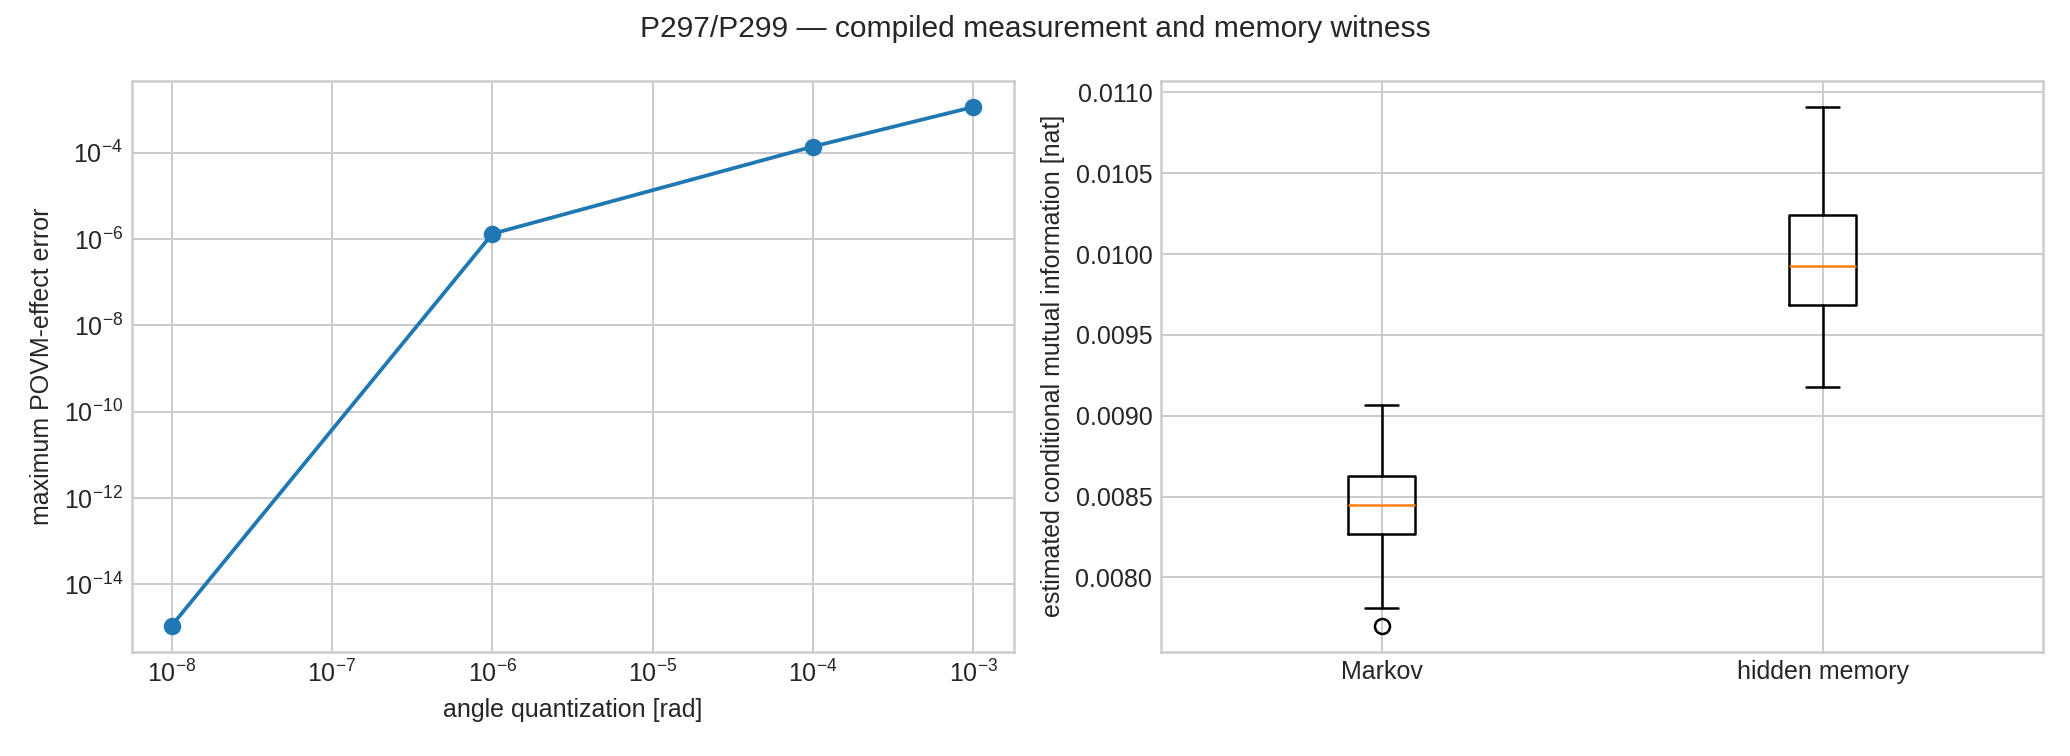
\includegraphics[width=0.97\textwidth]{FIN_Programs_295_308_Figures/p297_p299_mesh_memory.png}
\caption{Exact complex-unitary current-mesh compilation and a multitime memory witness.}
\end{figure}

\chapter{New theoretical objects O54--O61}

\section{O54 --- Spectral Observation Signature}

For a declared operational menu \(\mathcal C\), define

\[
\Sigma_{\mathcal C}(A)
=
\left\{
C_r^\ast(A+zI)^{-1}C_r,\;
p_A^c
:
r,z,c\in\mathcal C
\right\}.
\]

This object records only the pole/\allowbreak{}residue and outcome-law information visible to the declared probes, preparations, times, and instruments.

\textbf{Status:} \textbf{[Constructed]}. It is injective only under explicit cyclicity, visibility, and full-rank conditions.

\section{O55 --- Bernstein Spectral Completion}

The smallest monotone positive scalar subordination candidate is

\[
A_S=\Phi(A_L),
\]

where, for example,

\[
\Phi(\lambda)
=
b\lambda
+\sum_qc_q\frac{\lambda}{\lambda+r_q},
\qquad
b,c_q,r_q\ge0.
\]

Every such \(\Phi\) is increasing. P298 finds 32 mode-order inversions between the absolute-value-repaired legacy spectrum and the strict spectrum.

\textbf{Status:} \textbf{\statusRefuted{}} for the tested legacy-absolute to strict class.

\section{O56 --- Operational Prediction Pseudometric}

\[
d_{\mathcal C}(K,K')
=
\sup_{c\in\mathcal C}
\frac12\|p_K^c-p_{K'}^c\|_1.
\]

Two kernels may be pointwise different but operationally equivalent relative to a restricted menu. Conversely, a single operational witness can separate them without claiming a pointwise completion.

\textbf{Status:} \textbf{[Defined]}; only finite slices have been computed.

\section{O57 --- Positive Path-Scale Measure}

\[
h_\nu(d)=\int_0^\infty e^{-sd}\,d\nu(s),
\qquad \nu\ge0.
\]

The legacy envelope has

\[
d\nu_\beta(s)
=
\frac{1}{\beta}e^{-s/\beta}\,ds,
\]

equivalently the \(u\)-integral used above. The strict envelope with \(\eta=1.8\) lies outside this cone.

\textbf{Status:} legacy representation \textbf{\statusProven{}}; strict exclusion \textbf{\statusProven{}}.

This spatial result does not prove temporal non-Markovianity. It only excludes one positive mixture of exponential \emph{distance} attenuations.

\section{O58 --- Scale-Orbit Prediction Quotient}

For heat and Gibbs families,

\[
(A,t,T)\sim(cA,t/c,cT),\qquad c>0.
\]

Projective spectra and rescaled prediction laws live on the quotient. A clock, energy, or temperature standard selects a representative but is not generated by the quotient.

\textbf{Status:} finite invariance \textbf{\statusProven{}}.

\section{O59 --- Role-Transfer Certificate}

Define a certificate

\[
\mathsf{RT}
=
(B,R_L,R_S,\tau,\Pi),
\]

where \(B\) is a typed legacy-to-strict completion, \(R_L\) and \(R_S\) are role maps, \(\tau\) is the semantic transport, and \(\Pi\) certifies representation, operational, and scale invariance. The central square must commute:

\[
R_S\circ B=\tau\circ R_L.
\]

\textbf{Status:} certificate schema \textbf{[Constructed]}. No historical electroweak, electromagnetic, or gravity role passes it.

\section{O60 --- Pointed Operational Kernel Package}

\[
\mathfrak K_{\rm phys}
=
\begin{aligned}
(&K,\rho,A,\mathcal T,\mathcal P,\mathcal I,\\
 &\mathcal E,\mathcal R,t_0,\kappa).
\end{aligned}
\]

The entries are:

\begin{itemize}
\item 
kernel \(K\);

\item 
state \(\rho\);

\item 
generator \(A\);

\item 
clock/\allowbreak{}time family \(\mathcal T\);

\item 
preparation family \(\mathcal P\);

\item 
instruments \(\mathcal I\);

\item 
environment \(\mathcal E\);

\item 
event record \(\mathcal R\);

\item 
operational pointing/\allowbreak{}reference \(t_0\);

\item 
dimensional scale \(\kappa\).

\end{itemize}

This is the smallest package in this release that can state a physical prediction without silently omitting the observer, apparatus, or unit.

\textbf{Status:} \textbf{[Mathematically defined]}. FIN does not derive all entries.

\section{O61 --- Typed Legacy--Strict Completion Span}

\[
K_L
\xleftarrow{\ \pi_L\ }
\mathcal P
\xrightarrow{\ \pi_S\ }
K_S.
\]

The parent \(\mathcal P\) must keep the following components separately typed:

\[
\mathcal P
=
\begin{aligned}
(&\text{radial attenuation},\ \text{phase resource},\
\text{compression},\\
 &\text{sector state},\ \text{orientation/sign},\
\text{normalization},\\
 &\text{operational map}).
\end{aligned}
\]

A direct sum \(A_L\oplus A_S\) is excluded as a trivial parent. A valid span must contain cross-support structure, naturality, or an experimentally distinguishable common mechanism.

\textbf{Status:} \textbf{[Proposed bridge architecture]}, not a completed bridge.

\chapter{Program results P295--P308}

\section{P295 --- Multi-probe operator-valued Stieltjes recovery}

For three visible poles,

\[
S_r(z)
=
\sum_{j=1}^{3}\frac{w_{rj}}{z+\mu_j},
\qquad
w_{rj}\ge0,
\]

the poles are shared across probes and the residues are probe dependent.

The true positive poles were

\[
(1.1710910,\;1.5263637,\;1.8883092).
\]

\begin{center}
\begingroup\fontsize{7}{8.4}\selectfont
\setlength{\tabcolsep}{2.5pt}
\renewcommand{\arraystretch}{1.16}
\begin{longtable}{@{}p{0.127\textwidth}p{0.205\textwidth}p{0.169\textwidth}p{0.163\textwidth}p{0.196\textwidth}@{}}
\toprule
\textbf{Probes} & \textbf{Relative noise} & \textbf{Median max pole error} & \textbf{95\% max pole error} & \textbf{Median max residue error} \\
\midrule
\endhead
1 & \(10^{-4}\) & 0.4955 & 0.6617 & 0.0860 \\
4 & \(10^{-4}\) & 0.1502 & 0.4778 & 0.0425 \\
1 & \(10^{-3}\) & 0.6617 & 0.8081 & 0.3427 \\
4 & \(10^{-3}\) & 0.5538 & 0.6617 & 0.0861 \\
\bottomrule
\end{longtable}
\endgroup
\end{center}

The single-probe Jacobian has rank \(6\); the four-probe stacked Jacobian has rank \(15\), equal to the number of fitted parameters in each case.

\textbf{Verdict:} local injectivity \textbf{[Proven, conditional]}; frozen recovery \textbf{\statusStrong{}}. Full rank does not imply uniform minimax stability.

\section{P296 --- General staged elimination}

Let \(F(x,y,z)\) take values in a transitive ordered relation. If \(z_\star(x,y)\) is universally minimal for fixed \(x,y\), and \(y_\star(x)\) is universally minimal after the inner elimination, then

\[
F(x,y_\star,z_\star(x,y_\star))
\le
F(x,y,z)
\]

for every \(y,z\).

Lean 4.28 machine-checks this abstract theorem and the uniqueness of an attained minimum value under antisymmetry. Separately, 400 exact rational SPD \(3\times3\) matrices satisfy equality between nested and direct Schur elimination.

\textbf{Verdict:} \textbf{\statusProven{}}. The dependency-free Lean theorem is the general variational logic, not a complete Mathlib theorem for positive matrix blocks.

\section{P297 --- Complex-unitary compilation of the strict current POVM}

For six strict current effects \(E_y\),

\[
V
=
\begin{bmatrix}
\sqrt{E_1}\\
\vdots\\
\sqrt{E_6}
\end{bmatrix},
\qquad
V^\ast V=I_{12}.
\]

An orthonormal complement extends \(V\) to a \(72\times72\) complex unitary. A complex Givens decomposition uses 1,428 two-mode rotations.

\begin{center}
\begingroup\small
\setlength{\tabcolsep}{2.5pt}
\renewcommand{\arraystretch}{1.16}
\begin{longtable}{@{}p{0.265\textwidth}p{0.310\textwidth}p{0.284\textwidth}@{}}
\toprule
\textbf{Parameter quantization} & \textbf{Unit. reconstruction error} & \textbf{Max effect error} \\
\midrule
\endhead
exact & \(2.07\times10^{-15}\) & \(1.11\times10^{-15}\) \\
\(10^{-6}\) rad & \(3.27\times10^{-6}\) & \(1.33\times10^{-6}\) \\
\(10^{-4}\) rad & \(3.06\times10^{-4}\) & \(1.40\times10^{-4}\) \\
\(10^{-3}\) rad & \(3.04\times10^{-3}\) & \(1.16\times10^{-3}\) \\
\bottomrule
\end{longtable}
\endgroup
\end{center}

All quantized reconstructions remain unitary to numerical precision because the Givens parameters are quantized within a unitary parameterization.

\textbf{Verdict:} ideal compilation \textbf{\statusProven{}}; tolerance response \textbf{\statusStrong{}}. This is not a fabricated photonic chip, a loss map, or a detector calibration.

\section{P298 --- Scalar complement and Bernstein completion no-go}

A scalar lifted complement

\[
\widetilde A
=
E B E^\ast+\alpha(I-EE^\ast)
\]

forces an eigenvalue \(\alpha\) of multiplicity at least \(12-m\). The strict generator has maximum eigenvalue multiplicity two. Therefore \(m=6\) and \(m=3\) scalar complements cannot be unitarily equivalent to strict for any \(\alpha\).

The best projective residuals are nonzero, and the legacy-absolute/\allowbreak{}strict mode comparison has 32 order inversions. Since every Bernstein function is increasing, a monotone scalar functional calculus cannot repair them.

\textbf{Verdict:} exact scalar/\allowbreak{}Bernstein completion \textbf{\statusRefuted{}}. A non-scalar parent, anisotropic source, signed resource, or carrier transport is new structure.

\section{P299 --- Multitime memory ledger}

At calibrated step \(\tau=0.35\), compare:

\[
P=e^{-\tau A_S}
\]

with a persistent hidden-rate mixture using rates \(0.65\) and \(1.35\).

\begin{center}
\begingroup\small
\setlength{\tabcolsep}{2.5pt}
\renewcommand{\arraystretch}{1.16}
\begin{longtable}{@{}p{0.420\textwidth}p{0.420\textwidth}@{}}
\toprule
\textbf{Quantity} & \textbf{Result} \\
\midrule
\endhead
homogeneous conditional mutual information & \(-4.09\times10^{-17}\) nat \\
hidden-memory conditional mutual information & 0.00105689 nat \\
best one-step Markov joint-prediction TV & 0.0215679 \\
shots per replication & 80,000 \\
frozen classifier accuracy & 1.000 \\
\bottomrule
\end{longtable}
\endgroup
\end{center}

\textbf{Verdict:} finite Markov-order witness \textbf{\statusProven{}}; count audit \textbf{\statusStrong{}}. The hidden bath and rates were supplied.

\section{P300 --- Positive path-mixture and fixed-phase no-go}

On \(d=1,\ldots,6\), the strict weights are positive. The historical legacy cosine is negative at \(d=2,3,4,5\). A positive amplitude and positive denominator preserve those legacy signs; they cannot produce strict.

For

\[
h_\eta(d)=\frac{1}{1+d^\eta},
\]

\[
h_\eta''(d)
=
\frac{\eta d^{\eta-2}
\left[(\eta+1)d^\eta-(\eta-1)\right]}
{(1+d^\eta)^3}.
\]

When \(\eta=1.8\), this is negative near the origin. The tested value at half the inflection distance is \(-1.06970\).

The 80-point Gauss--Laguerre verification of the exact legacy mixture has maximum residual \(1.21\times10^{-14}\).

\textbf{Verdict:} positive fixed-phase distance-mixture bridge \textbf{\statusRefuted{}}.

\section{P301 --- External P241 intake}

The repository was scanned for a non-template bundle manifest, raw event records, custody metadata, and a frozen hold-out. Files with names suggesting external analyses exist in older lanes, but no bundle satisfied the P241 laboratory-event admission contract used here.

\textbf{Verdict:} \textbf{[Blocked by external evidence]}. P242 was not executed on synthetic substitutes.

\section{P302 --- Sequential detector design with nuisance tomography}

The synthetic categorical click model jointly estimates:

\[
\theta=(g,\eta_{\rm det},V,d_{\rm dark},c_{\rm xtalk}).
\]

Dark, balanced, crosstalk, contrast, and symmetric physics configurations were used. A grid search over displacement \(h\) maximized the Fisher log-determinant.

\begin{center}
\begingroup\small
\setlength{\tabcolsep}{2.5pt}
\renewcommand{\arraystretch}{1.16}
\begin{longtable}{@{}p{0.420\textwidth}p{0.420\textwidth}@{}}
\toprule
\textbf{Quantity} & \textbf{Result} \\
\midrule
\endhead
optimal tested \(h\) & 1.375 \\
Fisher rank & 5 \\
predicted gradient standard deviation & 0.0101464 \\
empirical gradient bias & 0.000599 \\
empirical gradient RMSE & 0.009063 \\
nominal 95\% coverage & 0.9833 \\
replications & 60 \\
\bottomrule
\end{longtable}
\endgroup
\end{center}

\textbf{Verdict:} \textbf{[Strong evidence, synthetic]}. The result is an experimental design, not a physical calibration.

\begin{figure}[htbp]
\centering
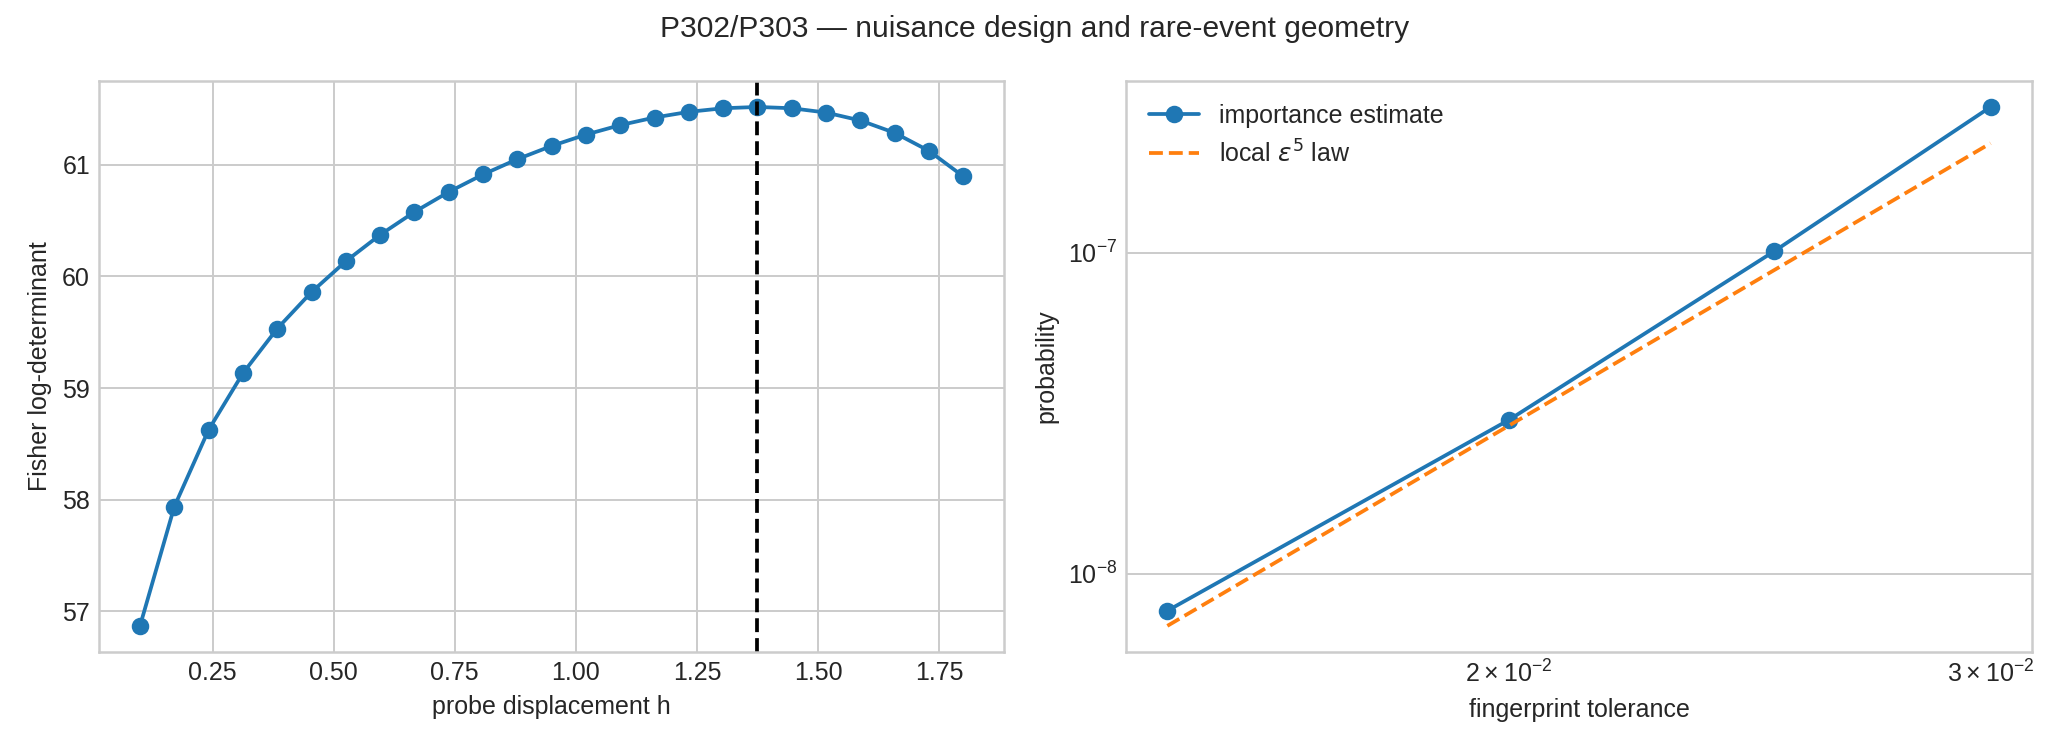
\includegraphics[width=0.97\textwidth]{FIN_Programs_295_308_Figures/p302_p303_detector_rare_event.png}
\caption{Joint detector nuisance design and strict-fingerprint rare-event geometry.}
\end{figure}

\section{P303 --- Local strict-fingerprint rarity}

Positive radial weights normalized to the simplex have five independent coordinates. The derivative of the sorted projective spectral fingerprint at strict has rank five and

\[
\det(J^\top J)=4880.98495.
\]

Under the uniform simplex null, the local small-ball law is

\[
\Pr(\|F(w)-F(w_S)\|\le\varepsilon)
\sim
\frac{5!\,\operatorname{Vol}(B_5)}
{\sqrt{\det(J^\top J)}}
\varepsilon^5.
\]

Importance sampling over \(\varepsilon=0.015,0.020,0.025,0.030\) gives fitted exponent \(5.217\).

\textbf{Verdict:} local exponent \textbf{\statusProven{}}; finite-tolerance comparison \textbf{\statusModerate{}}. Singular charts and global look-elsewhere effects remain outside the theorem.

\section{P304 --- Adversarial finite-time equivalence}

For observed times \(t_i\in\{0.15,0.35,0.65\}\), define

\[
\tau(t)
=
t+\epsilon t\prod_i(t-t_i)^2.
\]

The selected \(\epsilon\) gives

\[
0.99626\le\tau'(t)\le1.25
\]

on the tested interval, so

\[
A_{\rm alt}(t)=\tau'(t)A_S
\]

is a positive time-dependent rate. At every observed time,

\[
e^{-\tau(t_i)A_S}=e^{-t_iA_S}
\]

exactly, while the maximum off-grid vertex total-variation difference is \(0.002684\).

\textbf{Verdict:} unrestricted clock/\allowbreak{}mechanism identification from a finite time grid \textbf{\statusRefuted{}}. Homogeneity or a restricted clock family must be an explicit premise.

\section{P305 --- Intervention-assisted bridge-coordinate discovery}

The hypothetical coordinate

\[
K(\lambda)
=
(1-\lambda)\widehat K_{L,\lvert\cdot\rvert}
+\lambda\widehat K_S
\]

was supplied, together with the synthetic law

\[
\dot\lambda
=
0.55u-0.32\lambda-0.18\lambda^2.
\]

Passive data have library rank four. The intervention panel has joint rank six and recovers

\[
(0.55070,-0.31999,-0.18054)
\]

for the three nonzero coefficients. A new hold-out control has coordinate RMSE \(9.48\times10^{-6}\).

\textbf{Verdict:} identification method \textbf{[Strong evidence, synthetic]}; FIN interpretation \textbf{\statusSpeculative{}}. A coordinate-dependent law is not yet a natural completion theorem.

\begin{figure}[htbp]
\centering
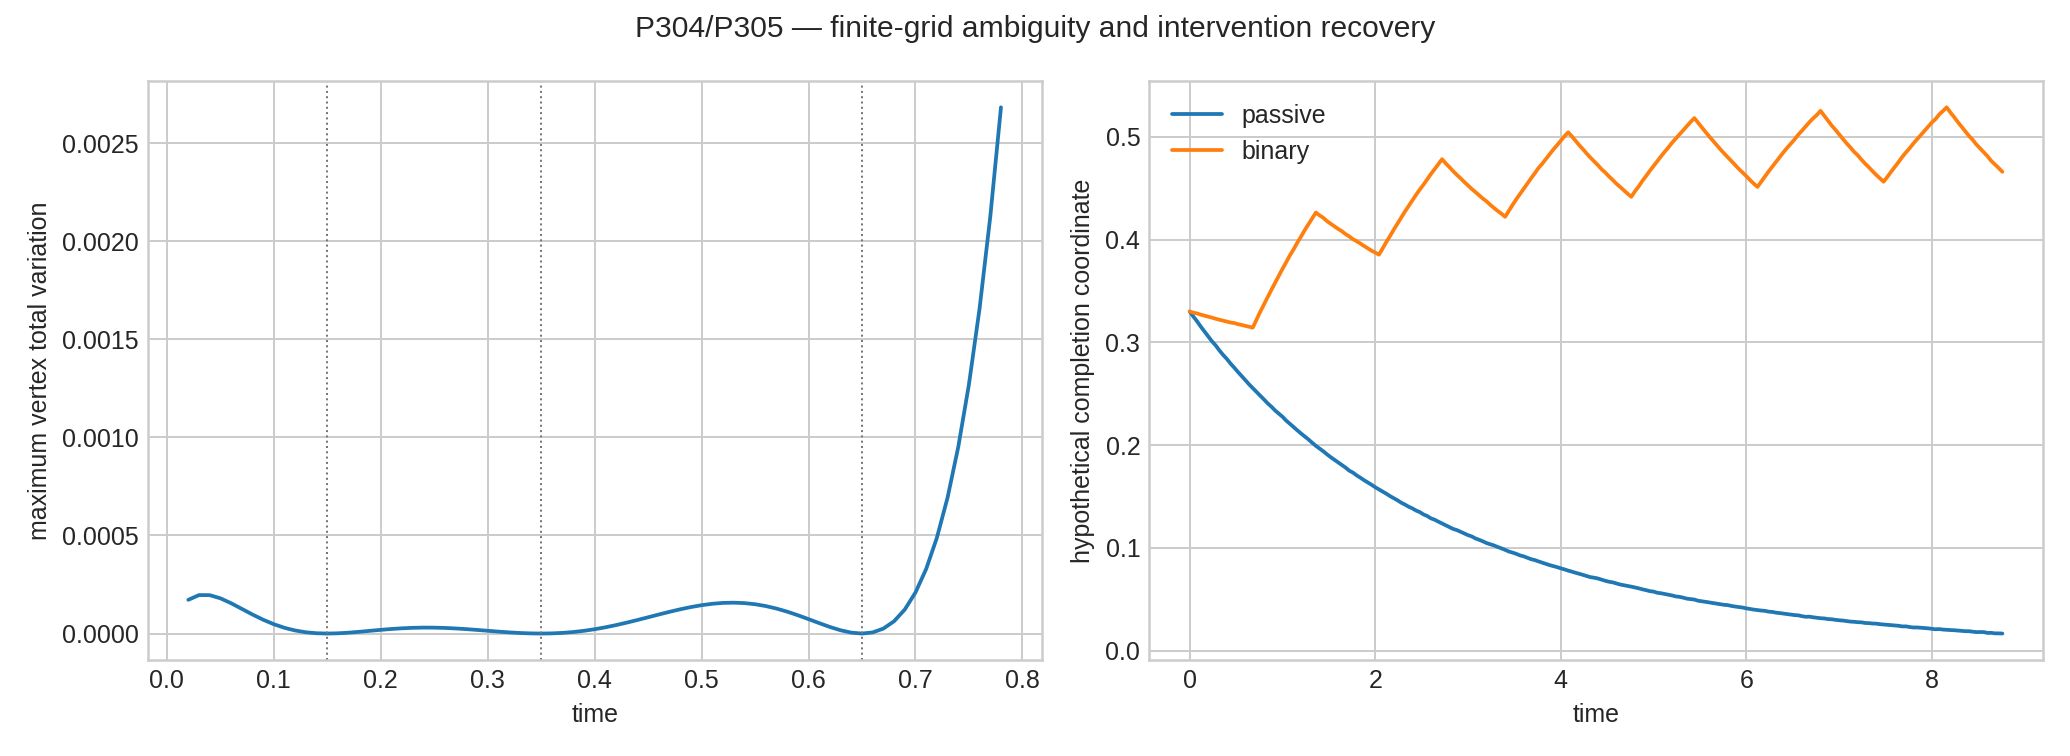
\includegraphics[width=0.97\textwidth]{FIN_Programs_295_308_Figures/p304_p305_clock_adaptation.png}
\caption{Finite-time clock ambiguity and intervention-assisted synthetic completion-coordinate recovery.}
\end{figure}

\section{P306 --- Physical reservoir evidence gate}

No independently certified hardware record was found with a calibrated clock, detector response, raw events, custody separation, and a preregistered hold-out.

\textbf{Verdict:} \textbf{[Blocked by external evidence]}. Reservoir simulations do not become hardware evidence by renaming their outputs.

\section{P307 --- Scale orbit and legacy-role invariance}

For \(c>0\),

\[
\operatorname{sig}(cA_S)=\operatorname{sig}(A_S),
\]

\[
e^{-t(cA_S)}=e^{-(ct)A_S},
\]

and the Gibbs law is unchanged under

\[
(A_S,T)\mapsto(cA_S,cT).
\]

The Fisher sensitivity to log generator scale and log clock conversion has rank one, with null direction \((1,-1)\).

Under a distance-coordinate change \(d'=cd\), the same legacy denominator is represented by

\[
\beta'=\frac{\beta}{c}.
\]

The old electroweak number is unchanged because it ignores \(\beta\), but it does not factor through a strict observable. The old electromagnetic formula varies by a factor \(20.39\) over the tested coordinate gauges; the \(\beta^{20}\) hierarchy varies by \(1.048576\times10^{26}\).

\textbf{Verdict:} unchanged electromagnetic and gravity role transfer \textbf{\statusRefuted{}}; electroweak transfer \textbf{[Blocked]}.

\section{P308 --- Pointed role-transfer theorem}

Lean proves:

\begin{enumerate}
\item 
a free nontrivial action has no globally invariant point;

\item 
two equivariant maps on a transitive torsor are equal if they agree at one supplied point.

\end{enumerate}

Finite cyclic torsors of order \(2\) through \(8\) have:

\begin{itemize}
\item 
zero invariant global sections;

\item 
\(n\) equivariant self-maps;

\item 
one pointed equivariant map.

\end{itemize}

None of the historical electroweak, electromagnetic, or gravity roles has all four certificate components: completion naturality, a strict observable, operational/\allowbreak{}scale invariance, and a dimensional anchor where required.

\textbf{Verdict:} pointed uniqueness \textbf{\statusProven{}}; physical-role transfer \textbf{[Blocked]}. QW-2191 remains open.

\begin{figure}[htbp]
\centering
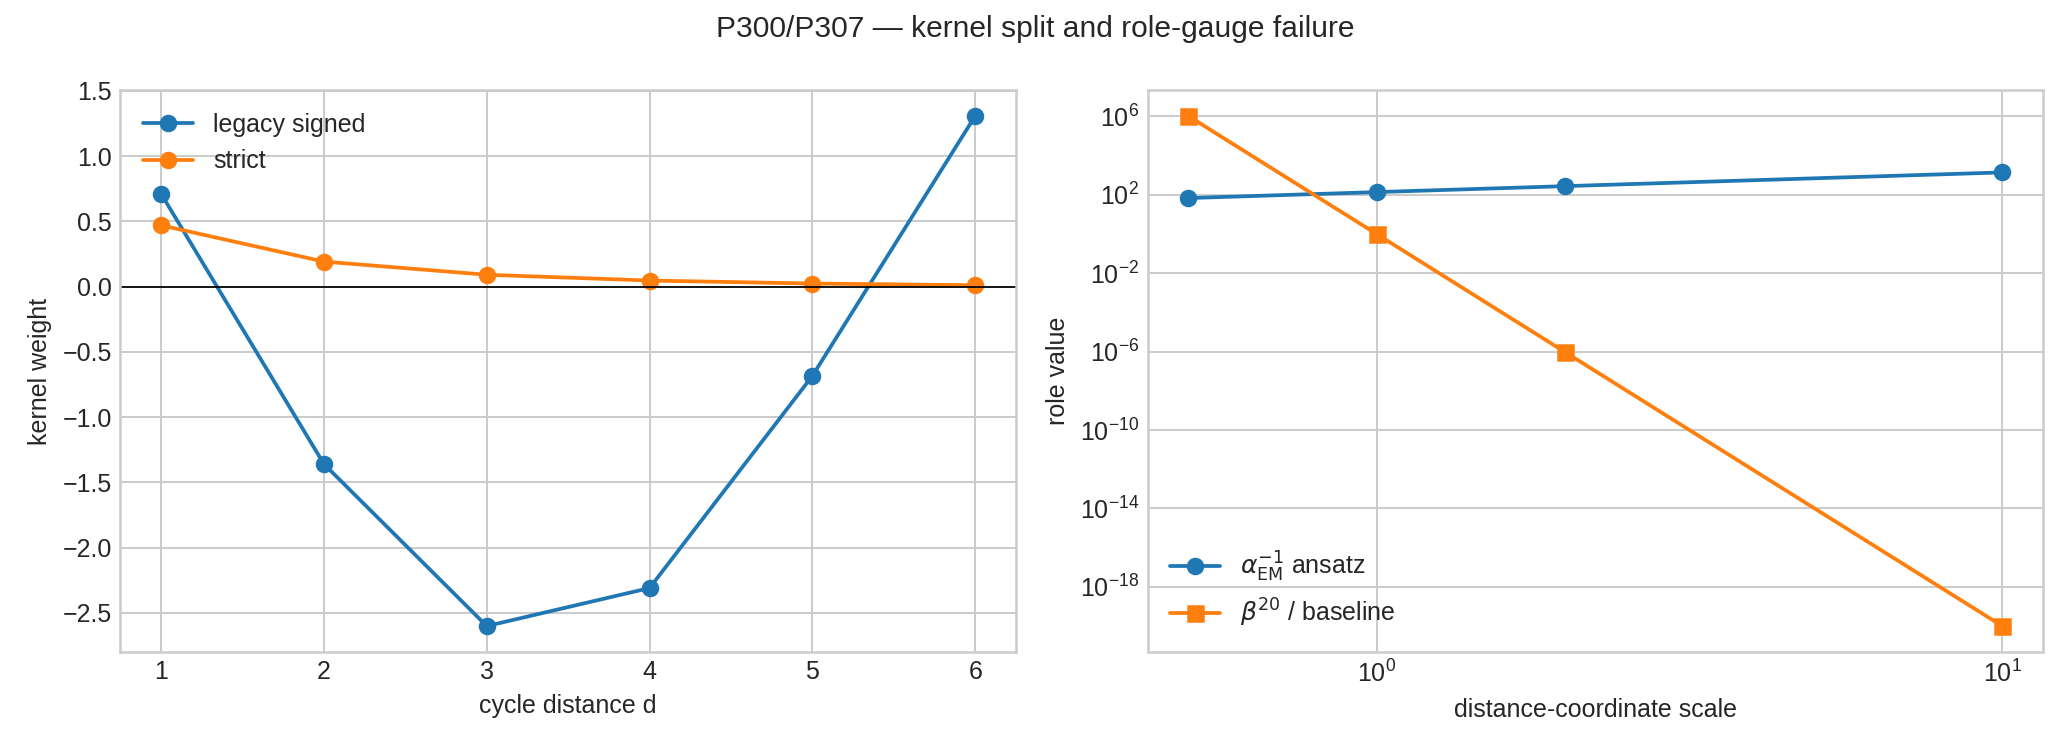
\includegraphics[width=0.97\textwidth]{FIN_Programs_295_308_Figures/p300_p307_kernel_role_invariance.png}
\caption{The legacy/strict kernel split and the coordinate-gauge failure of historical physical-role formulas.}
\end{figure}

\chapter{Cross-program synthesis}

\section{What survives from the old legacy intuition}

Three ideas survive, after correction.

First, the legacy kernel is a useful \textbf{long-range oscillatory carrier}. Its hyperbolic attenuation is not arbitrary: it is an exact positive mixture of exponential distance scales.

Second, the old decomposition anticipated that phase, attenuation, topology, and normalization should be separate ingredients. The modern strict analysis confirms that they cannot be collapsed into one scalar parameter.

Third, the historical physical formulas provide sharply defined benchmark maps that can be falsified. Their value is now methodological: they tell us which role-transfer diagrams must commute and which independent measurements would be needed.

\section{What does not survive}

The following inferences fail:

\[
\text{numerical agreement}
\not\Rightarrow
\text{operator-derived observable},
\]

\[
\text{dimensionless damping parameter}
\not\Rightarrow
\text{physical unit},
\]

\[
\text{legacy parameter role}
\not\Rightarrow
\text{strict physical role},
\]

\[
\text{positive path mixture}
\not\Rightarrow
\text{strict compression},
\]

\[
\text{spectral symmetry}
\not\Rightarrow
\text{selector or physical pointing}.
\]

\section{The new bridge hypothesis}

The smallest bridge still compatible with all no-go results is not a scalar formula \(K_S=f(K_L)\). It is a typed completion span

\[
K_L\leftarrow\mathcal P\rightarrow K_S
\]

combined with an operational quotient:

\[
\mathcal P
\longrightarrow
\Sigma_{\mathcal C}(A)
\longrightarrow
p(\text{record}\mid\text{preparation, clock, instrument}).
\]

At least one of the following must be genuinely new:

\begin{itemize}
\item 
a signed or complex interference measure;

\item 
a non-scalar common parent;

\item 
an anisotropic source;

\item 
a metric/\allowbreak{}carrier transport;

\item 
an independently prepared operational point;

\item 
a dimensional reference.

\end{itemize}

This is a necessity classification, not proof that any one candidate is realized.

\section{Why the old constants must bifurcate}

The old \(\alpha_{\rm geo}\) simultaneously served as:

\begin{itemize}
\item 
an information/\allowbreak{}fractal number \(4\ln2\);

\item 
a kernel amplitude;

\item 
an input to a physical coupling formula.

\end{itemize}

The old \(\beta_{\rm tors}\) simultaneously served as:

\begin{itemize}
\item 
a radial attenuation coefficient;

\item 
a hierarchy ratio;

\item 
an implicit scale converter.

\end{itemize}

P307 shows these identifications are not representation safe. The modern theory therefore requires \textbf{role bifurcation}:

\[
\alpha_{\rm geo}
\rightsquigarrow
(\alpha_{\rm info},\alpha_{\rm amplitude},\alpha_{\rm role}),
\]

\[
\beta_{\rm tors}
\rightsquigarrow
(\beta_{\rm shape},\beta_{\rm scale},\beta_{\rm role}),
\]

followed by explicit theorems if any components are to be reidentified.

\section{Deepest present interpretation}

The deepest interpretation surviving this round is:

\begin{quote}\itshape
FIN currently defines a finite spectral-information dynamics with a historically informative but incomplete bridge kernel. Its strict wave/\allowbreak{}diffusion duality and information-processing constructions are functional-calculus shadows of one positive generator. Turning that generator into physics requires a pointed operational kernel package and a role-transfer certificate. Neither the package nor the certificate follows from the radial kernel alone.

\end{quote}

\chapter{Failed approaches and impossibility boundaries}

\begin{center}
\begingroup\small
\setlength{\tabcolsep}{2.5pt}
\renewcommand{\arraystretch}{1.16}
\begin{longtable}{@{}p{0.291\textwidth}p{0.199\textwidth}p{0.370\textwidth}@{}}
\toprule
\textbf{Candidate} & \textbf{Result} & \textbf{Exact boundary} \\
\midrule
\endhead
positive fixed-phase damping & \statusRefuted{} & four sign mismatches \\
positive exponential distance mixture & [Refuted for strict] & strict envelope not completely monotone \\
scalar isotropic complement & \statusRefuted{} & forced flat-band multiplicity \\
Bernstein scalar functional calculus & \statusRefuted{} & 32 mode-order inversions \\
finite-time unrestricted mechanism ID & \statusRefuted{} & positive clock-warp counterexample \\
unchanged legacy EM role & \statusRefuted{} & coordinate-gauge dependence \\
unchanged legacy gravity role & \statusRefuted{} & coordinate-gauge dependence \\
electroweak role transfer & [Blocked] & no strict observable/\allowbreak{}factorization \\
selector from free symmetry & \statusRefuted{} & no invariant torsor point \\
laboratory confirmation & [Blocked] & no admitted independent event bundle \\
dimensional emergence & [Blocked] & scale orbit has no internal representative \\
\bottomrule
\end{longtable}
\endgroup
\end{center}

None of these scoped no-go results proves that no legacy-to-strict bridge or physical theory can exist. They prove that additional structure cannot remain implicit.

\chapter{Recommended Programs P309--P322}

Probabilities estimate the chance of a decisive result, including a rigorous no-go. They are planning judgments, not statistical posterior probabilities.

\begin{center}
\begingroup\fontsize{7}{8.4}\selectfont
\setlength{\tabcolsep}{2.5pt}
\renewcommand{\arraystretch}{1.16}
\begin{longtable}{@{}p{0.055\textwidth}p{0.090\textwidth}p{0.253\textwidth}p{0.320\textwidth}p{0.142\textwidth}@{}}
\toprule
\textbf{Rank} & \textbf{Program} & \textbf{Study} & \textbf{Decisive output} & \textbf{Probability} \\
\midrule
\endhead
1 & P309 & multi-probe Stieltjes minimax theorem & Le Cam/\allowbreak{}Cramér--Rao lower bound and optimal cyclic probes & 0.84 \\
2 & P310 & full formal Schur theorem & Mathlib proof for arbitrary finite positive block operators & 0.82 \\
3 & P311 & lossy complex-unitary mesh & dilation plus loss, detector confusion, phase drift, and robust distinguishability & 0.88 \\
4 & P312 & nontrivial common-parent SDP & construct or obstruct a cross-supported parent for \(C_{12},C_{16},C_{24}\) & 0.80 \\
5 & P313 & Mellin/\allowbreak{}regular-variation bridge audit & classify all positive path-counting laws compatible with the strict tail & 0.86 \\
6 & P314 & phase-resource theorem & test whether legacy torsion phase can naturally generate the strict non-torsion phase & 0.83 \\
7 & P315 & operational pseudometric/\allowbreak{}comb SDP & optimal preparation, time, and instrument separating legacy and strict & 0.78 \\
8 & P316 & minimal signed path-scale completion & quantify minimum negative/\allowbreak{}complex measure required to reproduce strict & 0.85 \\
9 & P317 & independent P241 admission & validate a real hash-committed event bundle without synthetic substitution & 0.30 \\
10 & P318 & Bayesian sequential detector drift & nuisance tracking, stopping rule, calibration transfer, and coverage under drift & 0.72 \\
11 & P319 & global coarea/\allowbreak{}look-elsewhere theorem & stratify eigenvalue-degeneracy charts and bound family-wise false positives & 0.69 \\
12 & P320 & restricted-clock experimental design & choose off-grid times/\allowbreak{}interventions that defeat the P304 warp class & 0.77 \\
13 & P321 & physical reservoir gate & preregister and execute an external hardware reservoir comparison & 0.28 \\
14 & P322 & single-role naturality certificate & attempt one complete strict electroweak role map; otherwise prove its obstruction & 0.61 \\
\bottomrule
\end{longtable}
\endgroup
\end{center}

\section{Recommended immediate sequence}

\[
\boxed{
P311
\longrightarrow
P316
\longrightarrow
P312
\longrightarrow
P315
\longrightarrow
P320
}
\]

This sequence:

\begin{enumerate}
\item 
converts the ideal P297 measurement into a realistic error model;

\item 
measures the extra signed/\allowbreak{}complex resource demanded by P300;

\item 
tests the smallest nontrivial common parent;

\item 
replaces pointwise resemblance with operational distinguishability;

\item 
designs a clock-sensitive falsification of the finite-time ambiguity.

\end{enumerate}

P317 and P321 must remain external gates. They should be executed only after real providers, registrars, calibrated apparatus, event records, and frozen hold-outs exist.

\chapter{Reproducibility}

\section{Executable artifacts}

\begin{itemize}
\item 
fin\_programs\_295\_308.py --- deterministic P295--P308 runner;

\item 
test\_fin\_programs\_295\_308.py --- regression and scientific-boundary suite;

\item 
FIN\_Programs\_295\_308\_Formal\_Core.lean --- dependency-free Lean 4.28 certificate;

\item 
FIN\_Programs\_295\_308\_Results.json --- machine-readable results;

\item 
FIN\_Programs\_295\_308\_Summary.csv --- program matrix;

\item 
eight detailed CSV tables;

\item 
five figures in FIN\_Programs\_295\_308\_Figures/\allowbreak{}.

\end{itemize}

The random seed is

\[
20260801.
\]

\section{Verification command}

Run python3 -m unittest -v test\_fin\_programs\_295\_308.py with the environment variable MPLCONFIGDIR=/\allowbreak{}tmp/\allowbreak{}mpl-fin.

Expected result: \textbf{17 tests passed, 0 failed.}

The suite recompiles the Lean certificate.

\section{Scientific boundary}

All detector, memory, adaptation, and finite-count data in this release are synthetic and are labeled as such. The external admission programs explicitly return blocked rather than manufacturing evidence.

\chapter{Final answer}

The old legacy work and the modern strict analysis do reveal one common mathematical story, but not the old physical one.

The common story is a transition from a positive multiscale oscillatory carrier to a localized positive spectral generator. The old hyperbolic attenuation has an exact path-scale-mixture interpretation. The strict attenuation, phase, and spectrum prove that this interpretation is insufficient. The missing object is therefore not another fitted constant. It is a typed operational completion containing a non-scalar or signed phase resource, a physical pointing, and a dimensional reference.

The deepest valid synthesis is:

\[
\boxed{
\begin{gathered}
\text{legacy carrier}
\;\xleftarrow{\ }\;
\text{typed completion parent}
\;\xrightarrow{\ }\;
\text{strict spectral generator}\\
\xrightarrow{\ \mathfrak K_{\rm phys}\ }
\text{testable outcome laws}
\end{gathered}
}
\]

The first two arrows remain incomplete; the last arrow requires operational and dimensional resources that are not generated by the kernel. Historical physical-role formulas may be retained only as preregistered hypotheses until they factor through this diagram and pass the Role-Transfer Certificate.

\chapter{References}

\begin{enumerate}
\item 
N. I. Akhiezer, \emph{The Classical Moment Problem}, Oliver \& Boyd, 1965.

\item 
C. Berg, J. P. R. Christensen, and P. Ressel, \emph{Harmonic Analysis on Semigroups}, Springer, 1984.

\item 
R. Bhatia, \emph{Positive Definite Matrices}, Princeton University Press, 2007.

\item 
S. N. Bernstein, "Sur les fonctions absolument monotones," \emph{Acta Mathematica} 52 (1929).

\item 
M.-D. Choi, "Completely positive linear maps on complex matrices," \emph{Linear Algebra and its Applications} 10 (1975).

\item 
M. G. Krein and A. A. Nudelman, \emph{The Markov Moment Problem and Extremal Problems}, AMS, 1977.

\item 
M. A. Nielsen and I. L. Chuang, \emph{Quantum Computation and Quantum Information}, Cambridge University Press, 2010.

\item 
M. Pollock et al., "Operational Markov condition for quantum processes," \emph{Physical Review Letters} 120 (2018).

\item 
W. F. Stinespring, "Positive functions on \(C^\ast\)-algebras," \emph{Proceedings of the American Mathematical Society} 6 (1955).

\item 
D. V. Widder, \emph{The Laplace Transform}, Princeton University Press, 1941.

\end{enumerate}


\clearpage
\chapter*{Reproduction certificate}
\addcontentsline{toc}{chapter}{Reproduction certificate}
\begin{Verbatim}[fontsize=\small]
MPLCONFIGDIR=/tmp/mpl-fin \
python3 -m unittest -v test_fin_programs_295_308.py
\end{Verbatim}
Expected result: 17 tests passed, 0 failed.  The suite recompiles the
dependency-free Lean 4.28 certificate.  Detector, memory, adaptation, and
finite-count studies are synthetic.  No independent P241 laboratory bundle
or certified hardware reservoir record was admitted.

\medskip
\noindent\textbf{Suggested citation:}

\.Zuchowski, K. (2026). \emph{FIN Research Programs P295--P308:
Legacy Physics Revisited---Positive Path Mixtures, Strict Spectral
Completion, and Physical-Role Transfer} (Release 10.27; Version 1.0.0)
[Preprint]. Zenodo.

\end{document}
